\section{Die Datenaufbereitung}\label{die datenaufbereitung}
Die vom Deutschen Wetterdienst (im Folgenden DWD abgekürzt) in fünf minütiger Auflösung bereitgestellten Radardaten, müssen für das Training der Netze und deren Vorhersage in ein Bildformat umgewandelt werden.  
Bei den bereits umgewandelten Bildern viel während der Entwicklung der Baseline auf, dass die Bilder weit weniger Regentage abbilden als es tatsächlich regnet. Daraufhin wurde das bisher vorgenommene Preprocessing evaluiert. Um die Radardaten in ein Bild umzuwandeln, muss jeder Radardatenpunkt in ein Pixelfarbwert transformiert werden. Bisher wurde dafür ein Sakalierungsfaktor berechnet mit dem jeder Radardatenpunkt multipliziert wurde. Der Faktor ergab sich aus dem zur Verfügung stehenden Wertebereich (0 bis 255), welcher durch den Maximalwert der Radardaten geteilt wurde. So erhält man transformierte Radarwerte in einem Bereich von 0 bis 255.  
Anschließend folgte eine Inspizierung der Daten. Hierfür wurde exemplarisch die Radardaten von Juni 2016 herangezogen. 

\begin{figure}[h]
 \centering
 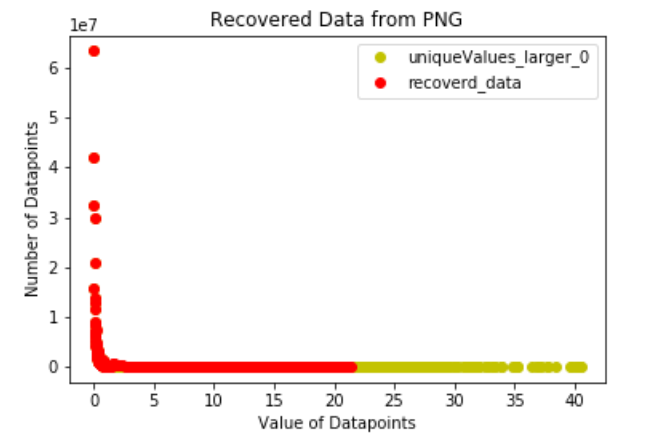
\includegraphics[width=0.6\textwidth,angle=0]{abb/datenaufbereitung_beispiel}
 \caption[Datenaufbereitung]{Hier muss eine Beschreibung hin.}
\label{fig:datenaufbereitung}
\end{figure}

Geplottet werden alle auftretenden Werte sowie dessen Häufigkeit. Hierbei stechen zwei Ausreißer hervor, welche sehr viel häufiger vorkommen als die restlichen Werte. Der Wert –9999 steht dabei dafür, dass keine Daten verfügbar sind und der zweite Ausreißer ist bei 0, was für “kein Regen” steht. In dem folgenden Plot werden die beiden Ausreißer gefiltert, da die relevanten Informationen in den restlichen Datenpunkten stecken.   

\begin{figure}[h]
 \centering
 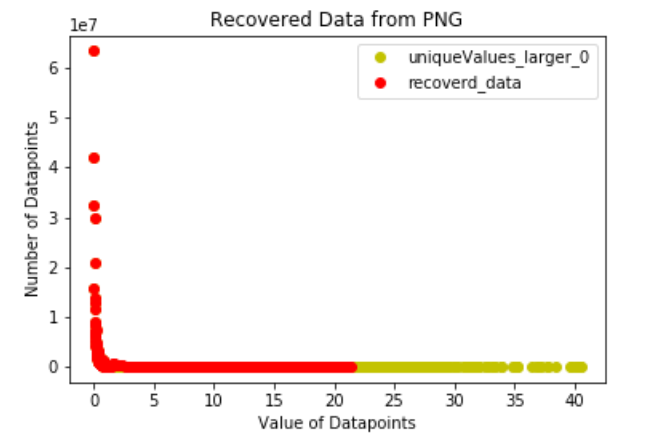
\includegraphics[width=0.6\textwidth,angle=0]{abb/datenaufbereitung_beispiel}
 \caption[Datenaufbereitung]{Hier muss eine Beschreibung hin.}
\label{fig:datenaufbereitung}
\end{figure}

In diesem Plot dargestellt sind die Radardaten bei denen es regnet. Es wird deutlich, dass ein Großteil der Datenpunkte klein ist. Der Mittelwert liegt bei 0,1744 und zeigt das Problem der bestehenden preprocessing Methode: Radardatenpunkte deren Wert auch nach der Multiplikation mit dem berechneten Skalierungsfaktor kleiner eins sind werden zu null. Aufgrund der vorliegenden Datenverteilung führt das zu einem erheblichen Fehler weshalb eine andere Methode entwickelt werden muss.   
Die beiden folgenden Plots zeigen verschiedene Perzentile und machen so die Datenverteilung deutlich.  

\begin{figure}[h]
 \centering
 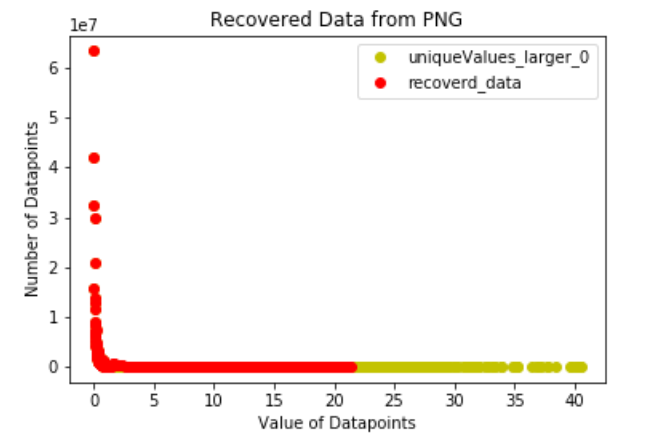
\includegraphics[width=0.6\textwidth,angle=0]{abb/datenaufbereitung_beispiel}
 \caption[Datenaufbereitung]{Hier muss eine Beschreibung hin.}
\label{fig:datenaufbereitung}
\end{figure}

\begin{figure}[h]
 \centering
 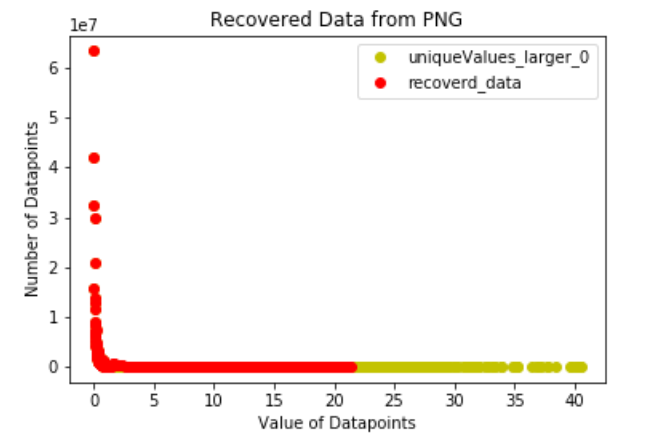
\includegraphics[width=0.6\textwidth,angle=0]{abb/datenaufbereitung_beispiel}
 \caption[Datenaufbereitung]{Hier muss eine Beschreibung hin.}
\label{fig:datenaufbereitung}
\end{figure}

Das 99 Prozent-Perzentil beinhaltet 138 verschiedene Werte. Wenn jedem dieser Werte ein Farbwert zugeordnet wird, werden 99 Prozent der daten bereits abgebildet und es verbleit ein Wertebereich von 117 mit welchem das letzte Prozent der Daten dargestellt werden kann.  
Der folgende Plot zeigt die Verteilung der noch verbleibenden Daten.

\begin{figure}[h]
 \centering
 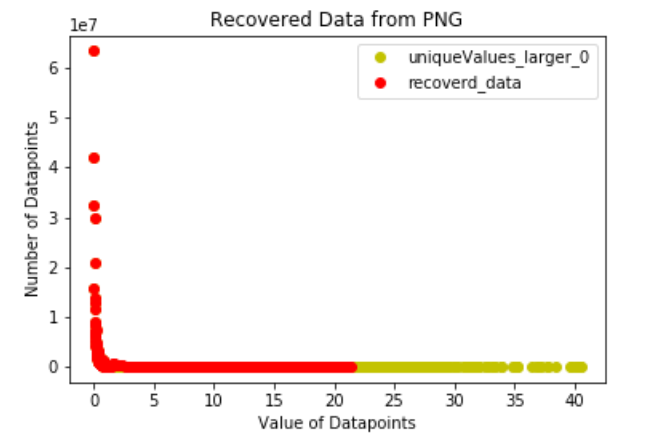
\includegraphics[width=0.6\textwidth,angle=0]{abb/datenaufbereitung_beispiel}
 \caption[Datenaufbereitung]{Hier muss eine Beschreibung hin.}
\label{fig:datenaufbereitung}
\end{figure}

Noch immer befindet sich der größte Teil der Datenpunkte im kleinem Wertebereich. Da für die verbleibenden Daten eine lineare Transformation ähnlich dem bereits bestehenden preprocessing Vorgang eingesetzt wird, entstehen Rundungsfehler. Da für die Berechnung des Skalierungsfaktors auch nicht der tatsächliche Maximalwert genutzt wird werden Werte die nach der Transformation über 255 sind auf 255 gesetzt. Diese Fehler sind verkraftbar, da es zum einen wichtiger ist alle Datenpunkte abzubilden und zum anderen die Auflösung der verschiedenen Regenstärken immer noch höher ist, als die der menschlichen Wahrnehmung.  
Radardaten welche transformiert werden müssen:  

\begin{figure}[h]
 \centering
 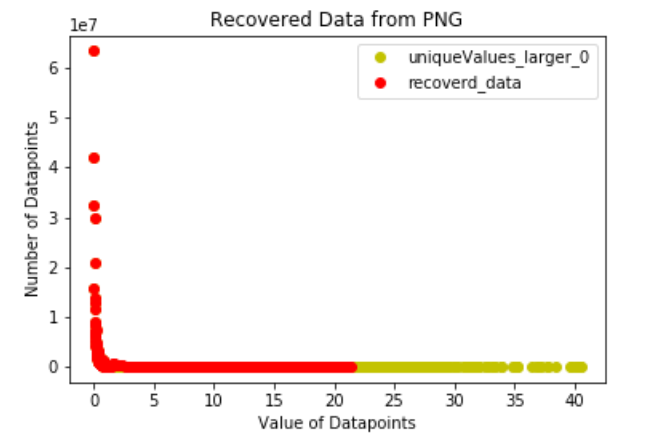
\includegraphics[width=0.6\textwidth,angle=0]{abb/datenaufbereitung_beispiel}
 \caption[Datenaufbereitung]{Hier muss eine Beschreibung hin.}
\label{fig:datenaufbereitung}
\end{figure}

Die transformierten Daten befinden sich in einem Wertebereich von 0 bis 255.  

\begin{figure}[h]
 \centering
 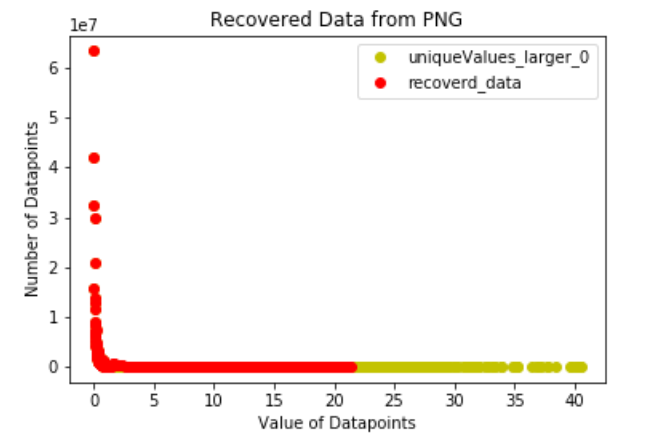
\includegraphics[width=0.6\textwidth,angle=0]{abb/datenaufbereitung_beispiel}
 \caption[Datenaufbereitung]{Hier muss eine Beschreibung hin.}
\label{fig:datenaufbereitung}
\end{figure}

Rekonstruiert man aus dem PNG Daten wieder die Radardaten ergibt sich der folgende Plot. Die quantitativ wiederhergestellte Anzahl der Datenpunkte beträgt 100%. Von den beschriebenen Fehlern macht sich im Plot vor allem letzterer im Plot bemerkbar. Werte größer als der für diesen Plot angenommenem Maximalwert von 21,39 wurden bei der Transformation auf 255 gesetzt und lassen sich daher nicht mehr konstruieren und erhalten deshalb den Wert 21,39.  

\begin{figure}[h]
 \centering
 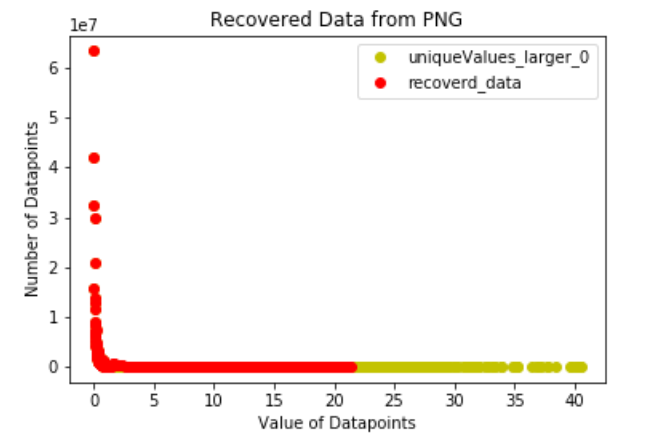
\includegraphics[width=0.6\textwidth,angle=0]{abb/datenaufbereitung_beispiel}
 \caption[Datenaufbereitung]{Hier muss eine Beschreibung hin.}
\label{fig:datenaufbereitung}
\end{figure}